\scanpage{11}
\figure{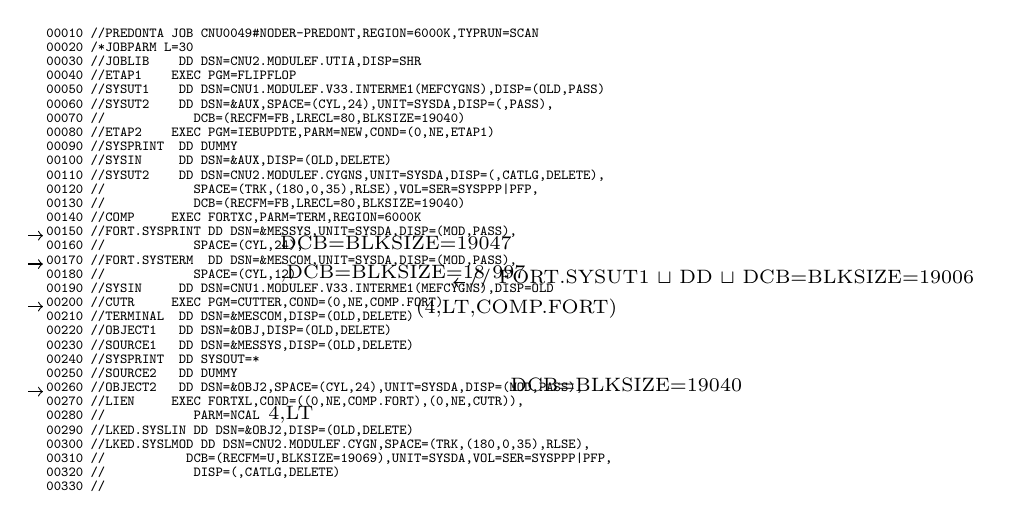
\begin{tikzpicture}[x=.075cm,y=.18cm]
\node[anchor=base west,inner sep=0pt,font=\tiny\ttfamily] at (0,0) {00010\ //PREDONTA\ JOB\ CNU0049\#NODER-PREDONT,REGION=6000K,TYPRUN=SCAN};
\node[anchor=base west,inner sep=0pt,font=\tiny\ttfamily] at (0,-1) {00020\ /*JOBPARM\ L=30};
\node[anchor=base west,inner sep=0pt,font=\tiny\ttfamily] at (0,-2) {00030\ //JOBLIB\ \ \ \ DD\ DSN=CNU2.MODULEF.UTIA,DISP=SHR};
\node[anchor=base west,inner sep=0pt,font=\tiny\ttfamily] at (0,-3) {00040\ //ETAP1\ \ \ \ EXEC\ PGM=FLIPFLOP};
\node[anchor=base west,inner sep=0pt,font=\tiny\ttfamily] at (0,-4) {00050\ //SYSUT1\ \ \ \ DD\ DSN=CNU1.MODULEF.V33.INTERME1(MEFCYGNS),DISP=(OLD,PASS)};
\node[anchor=base west,inner sep=0pt,font=\tiny\ttfamily] at (0,-5) {00060\ //SYSUT2\ \ \ \ DD\ DSN=\&AUX,SPACE=(CYL,24),UNIT=SYSDA,DISP=(,PASS),};
\node[anchor=base west,inner sep=0pt,font=\tiny\ttfamily] at (0,-6) {00070\ //\ \ \ \ \ \ \ \ \ \ \ \ DCB=(RECFM=FB,LRECL=80,BLKSIZE=19040)};
\node[anchor=base west,inner sep=0pt,font=\tiny\ttfamily] at (0,-7) {00080\ //ETAP2\ \ \ \ EXEC\ PGM=IEBUPDTE,PARM=NEW,COND=(0,NE,ETAP1)};
\node[anchor=base west,inner sep=0pt,font=\tiny\ttfamily] at (0,-8) {00090\ //SYSPRINT\ \ DD\ DUMMY};
\node[anchor=base west,inner sep=0pt,font=\tiny\ttfamily] at (0,-9) {00100\ //SYSIN\ \ \ \ \ DD\ DSN=\&AUX,DISP=(OLD,DELETE)};
\node[anchor=base west,inner sep=0pt,font=\tiny\ttfamily] at (0,-10) {00110\ //SYSUT2\ \ \ \ DD\ DSN=CNU2.MODULEF.CYGNS,UNIT=SYSDA,DISP=(,CATLG,DELETE),};
\node[anchor=base west,inner sep=0pt,font=\tiny\ttfamily] at (0,-11) {00120\ //\ \ \ \ \ \ \ \ \ \ \ \ SPACE=(TRK,(180,0,35),RLSE),VOL=SER=SYS\unsure{PPP|PFP},};
\node[anchor=base west,inner sep=0pt,font=\tiny\ttfamily] at (0,-12) {00130\ //\ \ \ \ \ \ \ \ \ \ \ \ DCB=(RECFM=FB,LRECL=80,BLKSIZE=19040)};
\node[anchor=base west,inner sep=0pt,font=\tiny\ttfamily] at (0,-13) {00140\ //COMP\ \ \ \ \ EXEC\ FORTXC,PARM=TERM,REGION=6000K};
\node[anchor=base west,inner sep=0pt,font=\tiny\ttfamily] at (0,-14) {00150\ //FORT.SYSPRINT\ DD\ DSN=\&MESSYS,UNIT=SYSDA,DISP=(MOD,PASS),};
\node[anchor=base west,inner sep=0pt,font=\tiny\ttfamily] at (0,-15) {00160\ //\ \ \ \ \ \ \ \ \ \ \ \ SPACE=(CYL,24),};
\node[anchor=base west,inner sep=0pt,font=\tiny\ttfamily] at (0,-16) {00170\ //FORT.SYSTERM\ \ DD\ DSN=\&MESCOM,UNIT=SYSDA,DISP=(MOD,PASS),};
\node[anchor=base west,inner sep=0pt,font=\tiny\ttfamily] at (0,-17) {00180\ //\ \ \ \ \ \ \ \ \ \ \ \ SPACE=(CYL,12)};
\node[anchor=base west,inner sep=0pt,font=\tiny\ttfamily] at (0,-18) {00190\ //SYSIN\ \ \ \ \ DD\ DSN=CNU1.MODULEF.V33.INTERME1(MEFCYGNS),DISP=OLD};
\node[anchor=base west,inner sep=0pt,font=\tiny\ttfamily] at (0,-19) {00200\ //CUTR\ \ \ \ \ EXEC\ PGM=CUTTER,COND=(0,NE,COMP.FORT)};
\node[anchor=base west,inner sep=0pt,font=\tiny\ttfamily] at (0,-20) {00210\ //TERMINAL\ \ DD\ DSN=\&MESCOM,DISP=(OLD,DELETE)};
\node[anchor=base west,inner sep=0pt,font=\tiny\ttfamily] at (0,-21) {00220\ //OBJECT1\ \ \ DD\ DSN=\&OBJ,DISP=(OLD,DELETE)};
\node[anchor=base west,inner sep=0pt,font=\tiny\ttfamily] at (0,-22) {00230\ //SOURCE1\ \ \ DD\ DSN=\&MESSYS,DISP=(OLD,DELETE)};
\node[anchor=base west,inner sep=0pt,font=\tiny\ttfamily] at (0,-23) {00240\ //SYSPRINT\ \ DD\ SYSOUT=*};
\node[anchor=base west,inner sep=0pt,font=\tiny\ttfamily] at (0,-24) {00250\ //SOURCE2\ \ \ DD\ DUMMY};
\node[anchor=base west,inner sep=0pt,font=\tiny\ttfamily] at (0,-25) {00260\ //OBJECT2\ \ \ DD\ DSN=\&OBJ2,SPACE=(CYL,24),UNIT=SYSDA,DISP=(MOD,PASS),};
\node[anchor=base west,inner sep=0pt,font=\tiny\ttfamily] at (0,-26) {00270\ //LIEN\ \ \ \ \ EXEC\ FORTXL,COND=((\deleted{0,NE},COMP.FORT),(0,NE,CUTR)),};
\node[anchor=base west,inner sep=0pt,font=\tiny\ttfamily] at (0,-27) {00280\ //\ \ \ \ \ \ \ \ \ \ \ \ PARM=NCAL};
\node[anchor=base west,inner sep=0pt,font=\tiny\ttfamily] at (0,-28) {00290\ //LKED.SYSLIN\ DD\ DSN=\&OBJ2,DISP=(OLD,DELETE)};
\node[anchor=base west,inner sep=0pt,font=\tiny\ttfamily] at (0,-29) {00300\ //LKED.SYSLMOD\ DD\ DSN=CNU2.MODULEF.CYGN,SPACE=(TRK,(180,0,35),RLSE),};
\node[anchor=base west,inner sep=0pt,font=\tiny\ttfamily] at (0,-30) {00310\ //\ \ \ \ \ \ \ \ \ \ \ DCB=(RECFM=U,BLKSIZE=19069),UNIT=SYSDA,VOL=SER=SYS\unsure{PPP|PFP},};
\node[anchor=base west,inner sep=0pt,font=\tiny\ttfamily] at (0,-31) {00320\ //\ \ \ \ \ \ \ \ \ \ \ \ DISP=(,CATLG,DELETE)};
\node[anchor=base west,inner sep=0pt,font=\tiny\ttfamily] at (0,-32) {00330\ //};

\draw[->] (-3,-14)--(-.5,-14);
\draw[->] (-3,-16)--(-.5,-16);
\draw[->] (-3,-19)--(-.5,-19);
\draw[->] (-3,-25)--(-.5,-25);
\node[anchor=base west,font=\scriptsize] at (38,-15) {\inserted{DCB=BLKSIZE=19047}};
\node[anchor=base west,font=\scriptsize] at (38,-17) {\inserted{,DCB=BLKSIZE=18 997}};
\node[anchor=base west,font=\scriptsize] at (70,-17.4) {\inserted{// FORT.SYSUT1 $\unsure{\sqcup}$ DD $\unsure{\sqcup}$ DCB=BLKSIZE=19006}};
\draw[<-] (69,-17.3)--(71,-17.3);
\node[anchor=base west,font=\scriptsize] at (61,-19.5) {\inserted{(4,LT,COMP.FORT)}};
\node[anchor=base west,font=\scriptsize] at (77,-25) {\inserted{DCB=BLKSIZE=19040}};
\node[anchor=base west,font=\scriptsize] at (36,-27) {\inserted{4,LT}};
\end{tikzpicture}}
\mspage{10}
